\documentclass[12pt]{article}
\usepackage{latexsym,amssymb,amsmath} % for \Box, \mathbb, split, etc.
% \usepackage[]{showkeys} % shows label names
\usepackage{cite} % sorts citation numbers appropriately
\usepackage{path}
\usepackage{url}
\usepackage{verbatim}
\usepackage{graphicx}
\usepackage{array}
\usepackage{multirow}

% horizontal margins: 1.0 + 6.5 + 1.0 = 8.5
\setlength{\oddsidemargin}{0.0in}
\setlength{\textwidth}{6.5in}
% vertical margins: 1.0 + 9.0 + 1.0 = 11.0
\setlength{\topmargin}{0.0in}
\setlength{\headheight}{12pt}
\setlength{\headsep}{13pt}
\setlength{\textheight}{625pt}
\setlength{\footskip}{24pt}

\renewcommand{\textfraction}{0.10}
\renewcommand{\topfraction}{0.85}
\renewcommand{\bottomfraction}{0.85}
\renewcommand{\floatpagefraction}{0.90}
\usepackage{graphicx}
\usepackage{wrapfig}
\usepackage{lscape}
\usepackage{rotating}
\usepackage{epstopdf}
\makeatletter
\setlength{\arraycolsep}{2\p@} % make spaces around "=" in eqnarray smaller
\makeatother

% change equation, table, figure numbers to be counted inside a section:
\numberwithin{equation}{section}
\numberwithin{table}{section}
\numberwithin{figure}{section}

% begin of personal macros
\newcommand{\half}{{\textstyle \frac{1}{2}}}
\newcommand{\eps}{\varepsilon}
\newcommand{\myth}{\vartheta}
\newcommand{\myphi}{\varphi}
\usepackage[utf8]{inputenc}

% Default fixed font does not support bold face
\DeclareFixedFont{\ttb}{T1}{txtt}{bx}{n}{8} % for bold
\DeclareFixedFont{\ttm}{T1}{txtt}{m}{n}{8}  % for normal

% Custom colors
\usepackage{color}
\definecolor{deepblue}{rgb}{0,0,0.5}
\definecolor{deepred}{rgb}{0.6,0,0}
\definecolor{deepgreen}{rgb}{0,0.5,0}
\definecolor{backcolour}{rgb}{0.96,0.96,0.96}

\usepackage{listings}

% Python style for highlighting
\newcommand\pythonstyle{\lstset{
		language=Python,
		basicstyle=\ttm,
		otherkeywords={self},             % Add keywords here
		keywordstyle=\ttb\color{deepblue},
		emph={MyClass,__init__},          % Custom highlighting
		emphstyle=\ttb\color{deepred},    % Custom highlighting style
		stringstyle=\color{deepgreen},
		frame=tb,                         % Any extra options here
		showstringspaces=false,            % 
		backgroundcolor=\color{backcolour}
}}


% Python environment
\lstnewenvironment{python}[1][]
{
	\pythonstyle
	\lstset{#1}
}
{}

% Python for external files
\newcommand\pythonexternal[2][]{{
		\pythonstyle
		\lstinputlisting[#1]{#2}}}

% Python for inline
\newcommand\pythoninline[1]{{\pythonstyle\lstinline!#1!}}

\newcommand{\IN}{\mathbb{N}}
\newcommand{\IZ}{\mathbb{Z}}
\newcommand{\IQ}{\mathbb{Q}}
\newcommand{\IR}{\mathbb{R}}
\newcommand{\IC}{\mathbb{C}}
\newcommand{\Real}[1]{\mathrm{Re}\left({#1}\right)}
\newcommand{\Imag}[1]{\mathrm{Im}\left({#1}\right)}
\usepackage{booktabs}
\usepackage{caption}
\usepackage{float}
\usepackage{titlesec}
\usepackage{capt-of}
%dashed line
\usepackage{array}
\usepackage{arydshln}
\setlength\dashlinedash{0.2pt}
\setlength\dashlinegap{1.5pt}
\setlength\arrayrulewidth{0.3pt}

%Widows & Orphans & Penalties

\widowpenalty500
\clubpenalty500
\clubpenalty=9996
\exhyphenpenalty=50 %for line-breaking at an explicit hyphen
\brokenpenalty=4991
\predisplaypenalty=10000
\postdisplaypenalty=1549
\displaywidowpenalty=1602
\floatingpenalty = 20000
\usepackage[T1]{fontenc}
\usepackage{fontspec}
\setmainfont[Scale=0.85, Ligatures={Required,Common,Contextual,TeX}]{TeX Gyre Schola} % Incredible font inside latex


\newcommand{\norm}[2]{\|{#1}\|_{{}_{#2}}}
\newcommand{\abs}[1]{\left|{#1}\right|}
\newcommand{\ip}[2]{\left\langle {#1}, {#2} \right\rangle}
\newcommand{\der}[2]{\frac{\partial {#1}}{\partial {#2}}}
\newcommand{\dder}[2]{\frac{\partial^2 {#1}}{\partial {#2}^2}}
\usepackage{enumitem}
\newcommand{\nn}{\mathbf{n}}
\newcommand{\xx}{\mathbf{x}}
\newcommand{\uu}{\mathbf{u}}
\usepackage{tikz}
\usetikzlibrary{arrows}
\usetikzlibrary{positioning}
\usepackage{titlesec}
\newcommand{\junk}[1]{{}}
\usepackage{sectsty}
\usepackage{xcolor}

\newcommand\MyBox[2]{
	\fbox{\lower0.75cm
		\vbox to 1.7cm{\vfil
			\hbox to 1.7cm{\hfil\parbox{1.4cm}{#1\\#2}\hfil}
			\vfil}%
	}%
}

\makeatletter
\renewcommand*\env@matrix[1][\arraystretch]{%
	\edef\arraystretch{#1}%
	\hskip -\arraycolsep
	\let\@ifnextchar\new@ifnextchar
	\array{*\c@MaxMatrixCols c}}
\makeatother

\makeatletter
\renewcommand*\env@matrix[1][*\c@MaxMatrixCols c]{%
	\hskip -\arraycolsep
	\let\@ifnextchar\new@ifnextchar
	\array{#1}}
\makeatother

\definecolor{darkblue}{rgb}{0,0,0.4}
\usepackage[colorlinks = true,
linkcolor = darkblue,
urlcolor  = darkblue,
citecolor = darkblue,
anchorcolor = darkblue]{hyperref}
% set two lengths for the includegraphics commands used to import the plots:
\newlength{\fwtwo} \setlength{\fwtwo}{0.45\textwidth}
% end of personal macros

\begin{document}
\DeclareGraphicsExtensions{.jpg}

\begin{center}
\textsc{\Huge Data Mining} \\[2pt]
	\textsc{\Large Assignment 2}\\
	\vspace{0.5cm}
  Ali Gholami \\[6pt]
  Department of Computer Engineering \& Information Technology\\
  Amirkabir University of Technology  \\[6pt]
  \def\UrlFont{\em}
  \url{http://ceit.aut.ac.ir/~aligholamee}\\
    \href{mailto:aligholamee@aut.ac.ir}{\textit{aligholamee@aut.ac.ir}}
\end{center}

\begin{abstract}
In this assignment, several paramount concepts of \textit{Data Analysis} will be explained. we'll discuss the importance of metrics in the first theoretical problem. A quick review on the \textit{Apriori} algorithm for the \textit{Association Rule Mining} will be explained also. We'll also show how \textit{Weka} can be used for \textit{Association Rule Mining}. Furthermore, The effectiveness of \textit{Normalization} concept is proposed. Finally, an \textit{Statistical} point of view will help us to demonstrate and rationalize the relationship between the \textit{Performance} of the \textit{Learning Algorithm} and the amount of \textit{Data} available. A chief section of this assignment is dedicated to solve the \textit{Titanic} problem, which is a great practice of data mining concepts in production. We'll use \textit{Python} programming language and three main libraries; \textit{Scikit-Learn}, \textit{Pandas} and \textit{Numpy} to tackle this problem. The Python implementation of the Titanic problem is provided on a \textit{Jupyter Notebook} attached with this report.
\end{abstract} 

\subparagraph{Keywords.} \textit{Apriori, Association Rule Mining, Normalization, Generalization, Preprocessing, Feature Engineering, Scikit-Learn, Pandas, Numpy, Python 3.5.}

\section{Data Preprocessing}
In this section, we'll be looking at our training data from different aspects. First, we need to get a quick intuition of how data looks like, how is that distributed and what to do with that! To do this, we'll be using some functions as described below.
\begin{python}
	separate_output('Training Data Types')
	print(train_data.dtypes)
\end{python}
In this part, we have printed the data types of our training set. Note that \textit{separate-output} is a self-defined function to make thing more clear in the terminal.
Now, its time for some statistics. To get a full understanding of how our numerical data is distributed, we use the following code.
\begin{python}
	separate_output('Statistical Information')
	print(train_data.describe())
\end{python}
The result of this part of code will be some statistical parameters such as: \textit{variance, mean, max, min, counts}. These can be useful in the future to make decisions about \textit{data normalization}.
Another amazing feature that \textit{Pandas} has provided for us is the ability to separately describe each column in the dataset. As an example, the first column contains $686$ missing values. Use the following code to believe this fact.
\begin{python}
	separate_output('Counts Values on a Column')
	print(train_data['col_1'].value_counts())
\end{python}
This column may not be seem much useful at the first glance, but we keep it since there are some good values for that column which might make it useful while we go further in the classification task.
Some of these columns are completely useless. Let's find them. The following function will return a dictionary consisting of number of missing values of each column.
\begin{python}
	def compute_nans(df):
	
	nans_dict = {}
	
	for col in df:
		nan_col_counter = 0
		for row in df[col]:
			if(row == '?'):
				nan_col_counter += 1
		nans_dict[str(col)] = [nan_col_counter]
	
	return nans_dict
\end{python}
We can obviously remove the following columns with more than 500 missing values.
\begin{python}
	cols_to_drop = [key for key, value in nan_cols.items() if value > 500]
	train_data = train_data.drop(cols_to_drop, axis=1)
\end{python}
Now its time to look for some \textit{correlation} between the features. We try to remove as much as correlated features as we can. There is a good reason for that. If two numerical features are perfectly correlated, then one doesn't add any additional information (it is determined by the other). So if the number of features is too high (relative to the training sample size), then it is beneficial to reduce the number of features. It's also important to mention that machine learning algorithms are very computationally intensive, and reducing the the features to independent components (or at least principal components) can greatly reduce the amount of resources required. Before implementing a dimensionality reduction approach on our data, let's make sure that the data is in the numeric form. But, before that, it is better to fill in the missing values with proper values.
\newpage
Here is the number of missing values for each column left in the training set.
\begin{python}
	{
		'col_12': 217,
		'col_2': 0,
		'col_3': 70,
		'col_32': 0,
		'col_33': 0,
		'col_34': 0,
		'col_35': 0,
		'col_37': 0,
		'col_39': 0,
		'col_4': 0,
		'col_5': 0,
		'col_7': 271,
		'col_8': 282,
		'col_9': 0
	}
\end{python}
There is only one numeric feature which is column 8 that its missing values can be filled using the mean of itself (column). To obtain this, we can use the following function to fill the missing values of an specific column.
\begin{python}
	train_data = train_data.replace('?', np.NaN)
	train_data.col_8 = train_data.col_8.astype(float)
	train_data['col_8'].fillna(train_data['col_8'].mean(), inplace=True)
\end{python}
The first line simply fixes the non-standard missing values given by dear T.A.s (just kidding bro :)). Then we change the type of column 8 to the float since \text{mean} function does not work for the \textit{int} types. Then we use the \textit{fillna} class member to fill the \textit{NaN} values with the average of that column.  Note that before continuing we shall extract the labels from our training data. We obtain this using the following code.
\begin{python}
	separate_output('Separated Training Labels')
	train_labels = train_data['col_39']
	train_data = train_data.drop(['col_39'], axis=1)
	print(train_labels)
\end{python}
Now the time for converting the categorical data to numeric form has come. We use the following function to 1. Convert the object types to categorical types 2. Convert all categorical types to numeric format.
\begin{python}
	def obj_to_num(df):
	
	for column in df.columns:
		if(df[column].dtype == 'object'):
			df[column] = df[column].astype('category')
			df[column] = df[column].cat.codes
	
	return df
\end{python} 
Now we perform a handy task called \textit{Standardization}. We can use either \textit{Standard Scaler} or \textit{Normalizer} to bring a unit \textit{L1} norm to the dataframe \textit{columns} or \textit{rows} respectively. In this case, we are going to use the \textit{Standard Scaler}.
\begin{python}
	train_data = StandardScaler().fit_transform(train_data)
\end{python}
This snippet will return a \textit{numpy} array of train data. Now we perform a \textit{Principal Component Analysis} to extract the best features depicting our dataset.
\begin{python}
	pca = PCA(n_components=5)
	pca.fit(train_data)
	train_data = pca.transform(train_data)
	test_data = pca.transform(test_data)
\end{python}
Now enough for the \textit{preprocessing} phase. In the next phase, I'll be digging through the \textit{Classification} using a \textit{Decision Tree} classifier.

\section{Classification}
\subsection{Decision Tree Classifier}
In this section, we first apply a simple decision tree on our training data.
\begin{python}
	decision_tree = DecisionTreeClassifier()
	decision_tree.fit(train_data, train_labels)
\end{python}
Of course, this is the simplest decision tree we can obtain right now. Nonetheless, we'll export the learned decision tree to watch it little bit! In the figure 2.1, we have provided a this decision tree. So, the time for evaluation has arrived. Let's evaluate the trained model on the training set first, then on the test set. We then perform various tweaks with the help of \textit{gridsearch} of \textit{Scikit} library. Note that the test set does not contain labels for the data, thus we are urged to use the \textit{train-test-split} function in order to break down the training set into 2 parts.
\begin{python}
	train_data, test_data, train_labels, test_labels =
	train_test_split(train_data, train_labels, test_size=0.2)
\end{python}
\subsection{Model Evaluation}
We fall into the evaluation section. Don't get nervous, we'll get back and try \textit{k-fold} cross validation also to improve the test results. Here is the demonstration of how we implemented the evaluation metrics.
\begin{python}
	prediction = decision_tree.predict(test_data)
	precision, recall, fscore, support = score(test_labels, prediction)
	classes = []
	[classes.append(x) for x in test_labels if x not in classes]
	for i in range(0, len(classes)):
	print('\nClass ', classes[i])
	print('     precision = {prec:4.2f}\%'.format(prec=precision[i]*100))
	print('     recall = {rc:4.2f}\%'.format(rc=recall[i]*100))
	print('     fscore = {fsc:4.2f}\%'.format(fsc=fscore[i]*100))
\end{python}
We first predict the labels for our test split of data. Then we calculate the scores using \textit{Sklearn.metrics}. We'll need to find the unique values in the test labels to display them in a beautiful way.
We are also planned to work with \textit{search-grid}. The evaluation metrics for the initial decision tree is given in the table 2.1.
\begin{table*}[!h] \centering
	%\ra{1.3}
	\begin{small}
		\begin{tabular}{@{}lrrrrrr@{}}\toprule
			\textbf{Metric/Class} & \textbf{'1'} & \textbf{'2'} & \textbf{'3'} & \textbf{'4'} & \textbf{'5'} & \textbf{'U'}\\ \midrule
			\textbf{Precision} & 100\% & 90\% & 100\% & NaN & 100\% & 99\%\\ \hdashline
			\textbf{Recall} & 83\% & 100\% & 100\% & NaN & 100\% & 99\%\\ \hdashline
			\textbf{F-Score} & 90\% & 94\% & 100\% & NaN & 100\% & 99\%\\ \hdashline
			\textbf{Support} & 6 & 9 & 2 & NaN & 17 & 126\\ \hdashline
			\bottomrule
		\end{tabular}
	\end{small}
	\caption{Measurements of the initial decision tree classifier without cross validation.}
\end{table*}
\subsection{K-Fold Cross Validation}
As there is never enough data to train your model, removing a part of it for validation poses a problem of underfitting. By reducing the training data, we risk losing important patterns in dataset, which in turn increases error induced by bias. So, what we require is a method that provides ample data for training the model and also leaves ample data for validation. K-Fold cross validation does exactly that. In K-Fold cross validation, the data is divided into k subsets. Now the holdout method is repeated k times, such that each time, one of the k subsets is used as the test set/ validation set and the other k-1 subsets are put together to form a training set. The error estimation is averaged over all k trials to get total effectiveness of our model. As can be seen, every data point gets to be in a validation set exactly once, and gets to be in a training set k-1 times. This significantly reduces bias as we are using most of the data for fitting, and also significantly reduces variance as most of the data is also being used in validation set. Interchanging the training and test sets also adds to the effectiveness of this method. As a general rule and empirical evidence, K = 5 or 10 is generally preferred, but nothing’s fixed and it can take any value\cite{cross_validation}. K-Fold splits the data to k parts and then for $i=1..k$ iterations does this: takes all parts except i'th part as the training data, fits the model with them and then predicts labels for i'th part (test data). In each iteration, label of i'th part of data gets predicted. In the end cross-val-predict merges all partially predicted labels and returns them as a whole.
\begin{python}
	decision_tree = DecisionTreeClassifier()
	NUM_FOLDS = 5
	predicted = cross_val_predict(decision_tree, train_data, train_labels, cv=NUM_FOLDS)
	scores = cross_val_score(decision_tree, train_data, train_labels, cv=NUM_FOLDS)
\end{python}
The accuracy of prediction is calculated and stored in the \textit{scores} variable. If we output the scores variable we'll get the following.
\begin{python}
	[0.95031056    0.99378882    0.99375    0.99367089    0.96815287]
\end{python}
This array displays the accuracy of prediction on each of these 5 folds. This part of the code integrates these values.
\begin{python}
	print("Accuracy: \%0.2f (+/- \%0.2f)" \% (scores.mean(), scores.std() * 2))
\end{python}
The mean of the accuracy is $98\%$.
\begin{sidewaysfigure}[!h]
	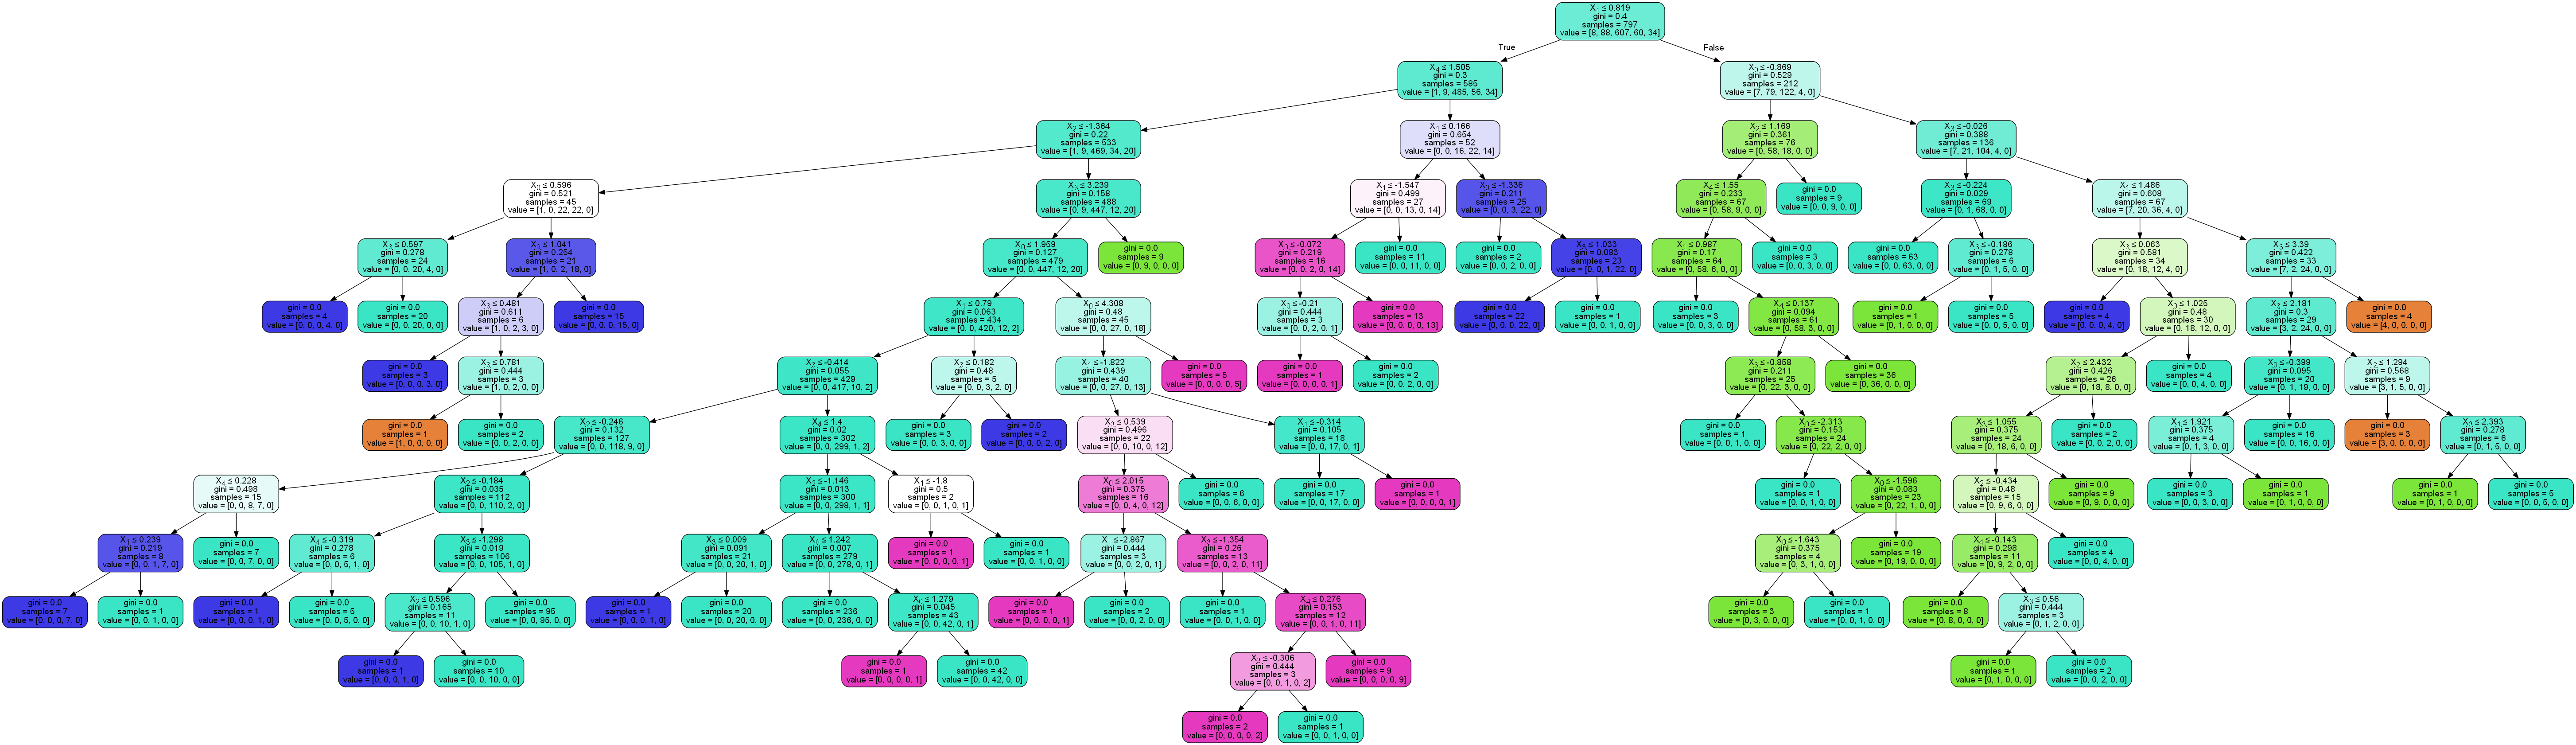
\includegraphics[width=\textwidth]{dt1.png}
	\caption{The First Lucky Decision Tree Trained on the Annealing Dataset.}
	\label{fig:PropProf}
\end{sidewaysfigure}
\begin{thebibliography}{999}
	
	\bibitem{cross_validation}
	Prashant Gupta,
	\emph{Cross-Validation in Machine Learning}.
	Towards Data Science,
	Jun 5, 2017.
	
\end{thebibliography}
\end{document}